% \title{Diffraction of Light}
% \author{An Introduction to Physics through Experiments}
% \date{}
% \maketitle

\chapter{Diffraction of Light}

\section*{Objectives}

\begin{enumerate}
    \item To determine the wavelength $\lambda$ of the light emitted by a laser source by studying the diffraction of light due to plane diffraction gratings.
    \item To determine the width of the given single slit by studying its diffraction pattern.
    \item To determine the diameter of a given wire by studying its diffraction pattern.
    \item To determine the size of the circular aperture by studying its diffraction pattern.
\end{enumerate}



\section*{Apparatus}

\begin{enumerate}
    \item A 10 mW semiconductor red laser source with a mount
    \item A 5 mW DPSS green laser source with a mount
    \item A set of plane diffraction gratings of different grating spacings with a holder and mounts
    \item A single helix (spring) set in a holder with a mount
    \item A double helix set in a holder with a mount
    \item Measuring tapes
    \item A set of screens 
    \item A single slit of fixed width mounted on a slide
    \item Two multiple slits and a set of circular apertures mounted on slides
    \item A spirit level
\end{enumerate}

\section*{Introduction}
	 
In \textit{Opticks} (1704), Issac Newton wrote, ``Light is never known to follow crooked passages nor to bend into the shadow''. He explained this by describing how particles of light always travel in a straight line, and how objects kept in the path of the light cast a shadow because the particles can never spread out behind the object. However, a set of experiments on the propagation of light through small apertures performed by Francesco Grimaldi, Augustine Fresnel, Thomas Young and a few others firmly established that light actually enters into the shadow region with a definite pattern when it passes through around an edge. The resulting pattern depends on the relative size of the aperture or obstacle and the wavelength of light. If the size is much larger than the wavelength, the bending will be almost unnoticeable. However, if the two are similar in size, the diffraction will be considerable.    
     
In this experimental problem, we will use a low power solid-state laser as a source of an intense beam of monochromatic light. When light from a distant source (or a laser source) passes around a thin aperture or through a narrow aperture and is then intercepted by a viewing screen, the light produces a pattern on the screen called a \textit{diffraction pattern}. When such a beam is incident on various diffracting components like a plane diffraction grating, a single slit, a wire mesh or a two-dimensional diffraction grating, the light emerging from these components show a variety of interesting diffraction patterns. This pattern consists regions of maximum and minimum intensities, which characterise the diffracting object. 

\section*{Theory}


\begin{imp}

\begin{center}
    \textbf{Babinet's Principle}
\end{center}

Two objects are called \textit{complementary} if one of them is transparent where the other is opaque and opaque where the other is transparent. An example of this is given in Figure (\ref{fig:complementary}).

\textbf{Babinet's principle} states that

\begin{center}
``Complementary objects \textbf{produce the same diffraction pattern}, except for the intensity of the central maxima.''
\end{center}

%This is a highly non-intuitive result, and one that you may study in some of your later courses. The mathematics of this are far beyond the scope of this lab session. 

Henceforth we will not differentiate between the patterns made by such complementary objects. We will thus speak of a single slit (or of a thin wire) having the `same' diffraction pattern, keeping in mind that the intensities of the central maxima are different.
\end{imp}

\begin{figure}[!htb]
    \centering
    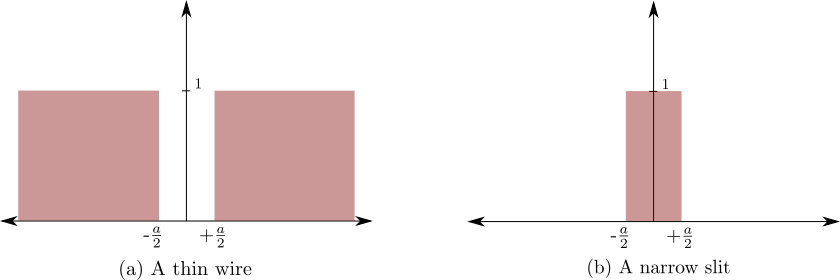
\includegraphics[scale=0.6]{figs/complementary.png}
    \caption{Transparency of a thin wire and of a single slit.}
    \label{fig:complementary}
\end{figure}

\begin{question}
\paragraph{Question:} What are the complementary objects of the following:

\begin{enumerate}
\item A transparent sheet of paper.
\item A circular aperture of diameter $d$.
\end{enumerate}
\end{question}



\subsection*{The Single Slit (or Thin Wire)}

When a (monochromatic) beam of light such as a laser is incident on a narrow single slit, the light emerging from the slit shows a diffraction pattern on a screen. The distribution of the intensity of light received on a screen show a pattern of varying intensity consisting of a bright central maximum with alternate minima and maxima of decreasing intensity on either side, known as a \textit{Fraunhofer diffraction pattern}.

Similarly, instead of a slit of width $a$, supposing we had a \textit{wire} of diameter $a$ placed as an obstruction to the laser beam. The resulting intensity pattern as observed on a screen almost exactly the same as that observed for a single slit. This intensity distribution can be written as a function of the angle $\theta$ as

\begin{equation*}
    I(\theta) = I(0) \left( \frac{\sin \beta}{\beta} \right)^2, \quad \quad  \beta = \frac{\pi a \sin \theta}{\lambda}
\end{equation*}

This function has been represented in Figure (\ref{fig:singleslit}).

\begin{figure}[!htb]
    \centering
    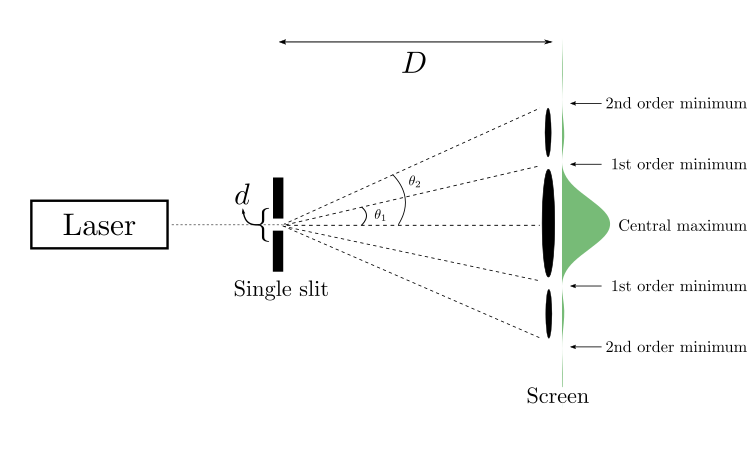
\includegraphics[width=0.75\textwidth]{figs/singleslit.png}
    \caption{The diffraction pattern produced by a single-slit aperture (or thin wire).}
    \label{fig:singleslit}
\end{figure}


Moving away from the central spot, when $\sin\beta=0$ (but $\beta \neq 0$), the intensity vanishes! The positions of these \textbf{minima} (zeros) of the intensity distribution pattern are given by the relation 

\begin{equation}
   a \sin{\theta_m} = \pm m \lambda  \quad\quad\quad \text{for    m  = 1, 2, 3,}\hdots,
   \label{singleslit}
\end{equation}

where $\lambda$ is the wavelength of the incident light, $a$ is the width of the slit and $\theta_m$ is the angle corresponding to $m$th minimum. Here the $\pm$ refers to either side of the central spot ($\theta = 0$).


\subsection*{The Double Slit}

We can now imagine two single slits of the same width next to each other. Such an arrangement is called a double-slit aperture. We could think of this aperture (shown in Figure (\ref{fig:doubleslit})) as a combination of a single slit of width $d$, and a thin wire of width $a$. 

This situation is slightly more complicated than the previous one; the thin obstacle of width $a$ will produce a diffraction pattern like the one in the previous section. However, the light from the two slits on either side will \textbf{interfere}, producing an overall interference pattern which also has its own maxima and minima! The mathematics of this is too difficult to understand right now; you will cover it in a later laboratory.

The resultant intensity distribution is given by   

\begin{equation}
    I(\theta) = I(0) \cos^2\delta \left( \frac{\sin \beta}{\beta} \right)^2, \quad \quad  \beta = \frac{\pi a \sin \theta}{\lambda}, \quad \delta = \frac{\pi d \sin \theta}{\lambda}
\end{equation}

For a screen placed at a large distance $D$ from the wire, the positions of the minima on the screen are observed at 

\begin{equation}
    \begin{aligned}
        x_{\pm n} = \pm n \frac{\lambda D}{a}, &\quad& \text{due to diffraction},\\
        x_{\pm m} = \pm \left( m - \frac{1}{2}\right) \frac{\lambda D}{d}, &\quad& \text{due to interference}
    \end{aligned}
    \label{doubleslit}
\end{equation}


\begin{figure}[!htb]
    \centering
    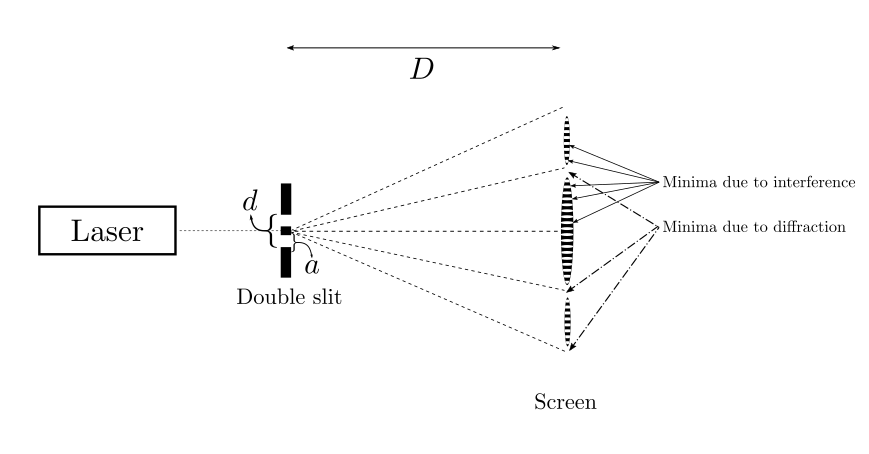
\includegraphics[width=0.75\textwidth]{figs/doubleslit.png}
    \caption{The diffraction pattern produced by a double-slit aperture is a combination of two patterns (diffraction due to a single wire and interference due to two slits).}
    \label{fig:doubleslit}
\end{figure}



\begin{question}
\paragraph{Question:} Look at the above condition for the fringes produced due to diffraction in Equation (\ref{doubleslit}). Is it different from the result obtained in the previous section (Equation (\ref{singleslit}))? If yes, why? If no, why not?
\paragraph{Question:} What is the ``complementary'' object to a double-slit?
\end{question}



\subsection*{Plane Diffraction Grating}

A transmission diffraction grating consists of a large number of slits separated from one another by an opaque region. The grating concentrates the diffracted light along a particular direction in contrast to the single slit, which has a rather broad diffraction maximum. The maxima (bright intense spots) produced by a grating are usually called the principal maxima. They are quite intense and are also widely separated; what cannot be detected visually are the large number of secondary maxima which lie between neighbouring principal maxima.

The expression, relating wavelength $\lambda$ of light used and the grating spacing $d$, with angle of deviation $\theta$ is
\begin{equation*}
    d \sin{\theta_m} = m \lambda,  \quad\quad\quad \text{for    m  = 1, 2, 3,}\hdots
\end{equation*}

In the above expression, $m$ represents the order of \textbf{maxima} points and the angle $\theta_m$  corresponds to  $m$th  order maximum intensity point. This relation is valid for a single slit and for the wire-like obstacle.

\begin{figure}[!htb]
    \centering
    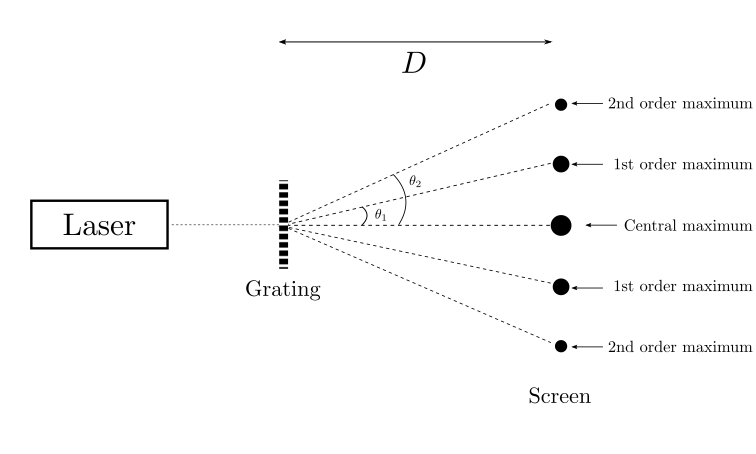
\includegraphics[width=0.75\textwidth]{figs/grating.png}
    \caption{The diffraction pattern produced by a plane diffraction grating.}
    \label{fig:grating}
\end{figure}


\subsection*{The Circular Aperture}

The diffraction pattern due to a circular aperture (known as an \textit{Airy diffraction pattern}) is similar to a single slit diffraction but the mathematics involved is more complicated which gives the expression nearly identical to that of the single slit. Hence we may apply the same expression to the diffraction due to a circular aperture, 

\begin{equation*}
    d \sin{\theta_m} = \overline{m} \lambda,  \quad\quad\quad \text{for    m  = 1, 2, 3,}\hdots
\end{equation*}

where $d$ is the diameter of the circular aperture and $\theta_m$ is the angle of deviation for the $m$th dark ring. The variable $\overline{m}$ has the following values:

\begin{equation*}
    \begin{aligned}
        m = 1 &\quad& \overline{m}=1.22\\
        m = 2 &\quad& \overline{m}=2.23\\
        m = 3 &\quad& \overline{m}=3.23\\
        m = 4 &\quad& \overline{m}=4.24\\
    \end{aligned}
\end{equation*}

\subsection*{Single and double helices:}
  
\begin{figure}[!htb]
    \centering
    \begin{subfigure}[b]{0.45\textwidth}
                \centering
                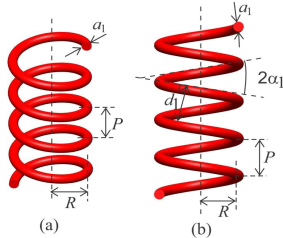
\includegraphics[width=0.75\textwidth]{figs/singlehelix.png}
                \caption{Schematic of a single helix (like RNA)}
                \label{fig:singlehelix1}
        \end{subfigure}%
        \begin{subfigure}[b]{0.45\textwidth}
                \centering
                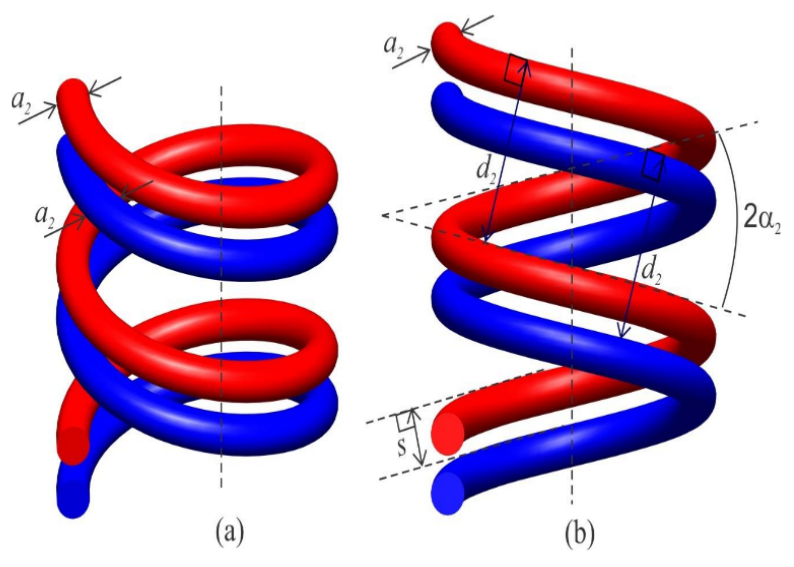
\includegraphics[width=0.75\textwidth]{figs/doublehelix.png}
                \caption{Schematic of a double helix (like DNA)}
                \label{fig:doublehelix1}
        \end{subfigure}
\end{figure}

Now consider a set of four identical wires, the net intensity distribution is a combination of diffraction from each wire and interference due to pairs of wires and hence depends on $a$, $d$ and $s$ (see Figure \ref{fig:fourwires}).

In other words, the combination of three different intensity patterns is observed.

\begin{figure}[!htb]
    \centering
    \begin{subfigure}[b]{0.45\textwidth}
                \centering
                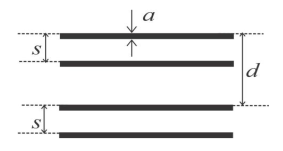
\includegraphics[width=0.75\textwidth]{figs/fourwires.png}
                \caption{Projection of four identical wires}
                \label{fig:fourwires}
        \end{subfigure}%
        \begin{subfigure}[b]{0.45\textwidth}
                \centering
                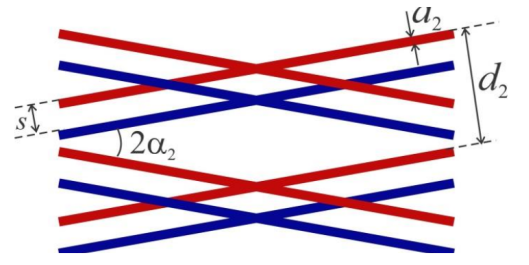
\includegraphics[width=0.75\textwidth]{figs/doublehelix-schema.png}
                \caption{The double helix given in the sample.}
                \label{fig:doublehelix2}
        \end{subfigure}
        \caption{Diffraction patterns of obstacles with three length scales.}
\end{figure}

\section*{Description}

In \textbf{Part A}, you will determine the wavelength of light of a laser using a set of diffraction gratings.

In \textbf{Part B}, you will use the laser whose wavelength you have just determined to measure the width of a single slit.

In \textbf{Part C}, you will study diffraction pattern of a circular aperture.

In \textbf{Part D (\textit{optional})}, you will study the diffraction pattern of a single helix.

In \textbf{Part E (\textit{optional})}, you will study the diffraction pattern of a double helix.


\section*{Procedural Instructions}

\subsection*{Part A}

Observe effect of colour and also of white light on the diffraction pattern obtained by a suitable grating. Then choose an appropriate diffraction grating and perform the measurements to determine the wavelength $\lambda$ of the laser. 

\begin{question}
\paragraph{Question:} Estimate the error in the value of the wavelength of light.

\paragraph{Question:} What are the sources of error in the above-determined value of $\lambda$? What measures should be taken to minimise these errors? 

\paragraph{Question:} Tilt the grating at an angle. How does this affect the diffraction pattern?
\end{question}

Now repeat this procedure for different gratings (with different values of $d$), and calculate wavelength $\lambda$ as accurately as possible.

\subsection*{Part B}

Design and perform the necessary experiment with a single slit of fixed width and determine the width d of the given single slit.

\begin{question}
\paragraph{Question:} Tilt the slit at an angle. How does this affect the diffraction pattern?
\end{question}


\subsection*{Part C}

Now take the given circular aperture as the diffracting object and determine the diameter of the circular aperture.

\subsection*{Part D}

Study of the diffraction pattern due to a helical spring and determine pitch of the spring and thickness of its wire. 


\begin{question}
\paragraph{Question:} Can you explain the form of the diffraction pattern observed? Does this part of the experiment relate in any way to Part B? 
\end{question}

\subsection*{Part E}

Study of the diffraction pattern due to a double helix (as in our DNA) and determine all its parameters, as shown in Figure (\ref{fig:doublehelix2}).

\begin{question}
\paragraph{Question} Describe the diffraction pattern obtained if you use a laser source to illuminate
\begin{enumerate}[label=(\alph*)]
    \itemsep0em
    \item A fine wire mesh,
    \item A square aperture,
    \item A rectangular aperture.
\end{enumerate}
\end{question}



\subsection*{Precautions}

\begin{enumerate}
    \item Never look directly at a laser beam with the naked eye. It may damage the eye permanently.
    \item Never point the laser at anyone else, for the same reason.
    \item Never point an optical device at a laser beam. It could damage the internal sensors.
    \item Never place highly reflective objects (such as rings, watches, and glassware) in the path of the laser beam.
    \item For proper working of laser, it should be kept on throughout. Do not put it off until you complete all your readings, but if you do not need the laser beam for measurements or alignment, use a light-blocking screen to block the  beam.
    \item Treat the laser source as you would any other electrical device: It should never be tampered with while the power cord is connected.
\end{enumerate}


\section*{References}

\begin{enumerate}
\itemsep0em
    \item Eric Stanley, Am. J. Phys., Vol.- 54, No.-10, October 1986, pp. 952.
    \item F.A. Jenkins, H.E. White, \textit{Fundamentals of Optics}, Third Edition, Mc-Graw Hill Kogakusha Ltd., Toyko, Japan, 1957, pp. 288-309, 328-350.
    \item F.W. Sears, \textit{Optics}, Third Edition, Asia Publishing House, 1958, pp 221-252.
    \item R.W. Ditchburn, \textit{Light}, Second Edition, The English Language Book Society and Blackie \& Son Ltd., 1963, pp 162-237.
    \item John Beynon, \textit{Introductory University Optics}, Prentice-Hall of India Pvt. Ltd., New Delhi (India), 1998, pp 158-190.
    \item Rajpal S. Sirohi, \textit{Wave Optics and its Applications}, Orient Longman Limited, (India), 1993, pp 169-210.
\end{enumerate}



\newpage